\documentclass[12pt,oneside]{article}
\usepackage{makeidx,anysize,mflogo,xspace,float,epsfig,url}
\usepackage{amsmath,amsfonts,amssymb,a4wide} 
\usepackage[utf8]{inputenc}
%\usepackage[francais]{babel}
%\usepackage[french]{babel}
\urlstyle{sf}
%\usepackage{subcaption}
\usepackage{hyperref}
\usepackage{graphicx}
\usepackage{graphics}
\usepackage{float}
\usepackage{caption}
\usepackage{colordvi} %??
\usepackage{listings} 
\usepackage{subfigure}
\usepackage{subfloat}
\usepackage{xcolor}
\graphicspath{{./figures/}}
%\usepackage[labelsep=quad,indention=10pt]{subfig}
\definecolor{grey}{rgb}{0.95,0.95,0.95} % on définit la couleur grise
	% (c'est un gris très clair)
	\definecolor{red}{rgb}{1.0,0.0,0.0} 
	\definecolor{green}{rgb}{0.0,1.0,0.0}
	\definecolor{blue}{rgb}{0.0,0.0,1.0}
	\lstloadlanguages{bash,Java,C,C++,csh,make,sh}%%[Visual]Basic,xml}
	\lstset{frame=none,basicstyle=\footnotesize,breaklines,tabsize=2,captionpos=b,
		prebreak={\hbox{$\rightarrow$}},postbreak={\hbox{$\hookrightarrow$}},
		showstringspaces=false,backgroundcolor=\color{grey}\bfseries,
		keywordstyle=\color{blue},commentstyle=\color{green}\textit,
		stringstyle=\color{red}\ttfamily,abovecaptionskip=2pt,aboveskip=0pt,
		belowskip=0pt,belowcaptionskip=0pt,numbers=none,columns=fullflexible, backgroundcolor=\color{grey}}
%left,numberstyle=\footnotesize,
%		stepnumber=2,numbersep=1pt}

\begin{document}


\begin{center}
{\bf \Large Redpitaya: fourth example} \\ \ \\
G. Goavec-M\'erou, J.-M Friedt \\ \ \\ \today
\end{center}

This tutorial is a sequel to the second one on which it is based. In addition to 
copying the ADC inputs to the DAC outputs, we wish (Fig. \ref{obj}) to {\bf mix} the stream of 
data coming from the ADC with a local numerically controlled oscillator ({\bf NCO}) 
(Fig. \ref{fin}).

\begin{figure}[h!tb]
\begin{center}
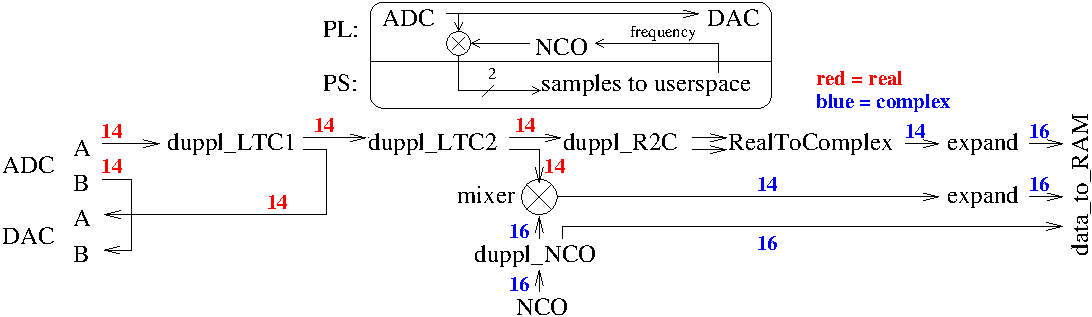
\includegraphics[width=\linewidth]{objective}
\caption{Top: general objective of the frequency transposition of the input signal, and bottom the
detailed list of blocks and data path width along the signal processing chain. Colored
numbers indicate datawidth, with red being real-valued streams and blue being 
complex-valued streams.}
\label{obj}
\end{center}

\hspace*{-1.5cm}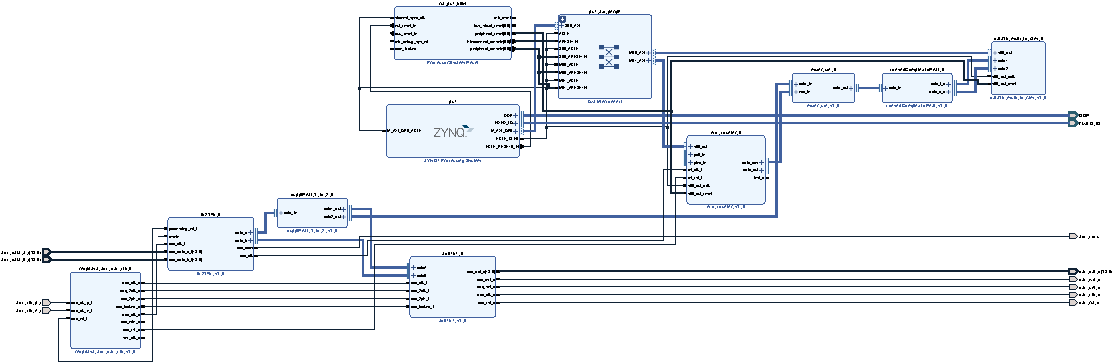
\includegraphics[width=1.2\linewidth]{design_1.pdf}
\caption{Schematic of the objective and final processing chain described in this document}
\label{fin}
\end{figure}

\section{NCO configuration}

The ADC to DAC and ADC to RAM blocks are the same as before, with stream
dupplication every time a new datastream must reach two users. The novely
is now the use of a NCO and mixer. The NCO accepts as a 32-bit (counter size) 
argument the normalized frequency, and outputs a 16-bit counter value. The
new challenge lies in handling varying data sizes: the ADC outputs 14-bit data
readily accepted by the DAC and the mixer input (whose input data size is defined
as 14-bit wide while the NCO port is set to 16-bit width) but the Data to RAM block
can only handle a single data size on all input ports. The option is either to
degrade the 16-bit NCO to 14-bit, or to expand the 14-bit ADC and mixer outputs
to 16-bits. The latter option was selected to introduce the
``expanderComplex'' (its application to real valued streams named ``expanderReal'' 
is also available) whose function is to add missing Most Significant bits to the 
input stream to match the expected output stream data size.

Since we feed the Data to Ram block with 3 streams of complex data (real and imaginary) each 
encoded as 16-bit values, we must read 12-bytes for each new dataset. Hence, in the
userspace application, the dataset transfered from the FPGA to the RAM is 12 times the
RAM size which is set to 4096 samples.

\section{PS: Linux kernel driver}

The same driver for communicating with the PL will be requested as before
({\tt data\_to\_ram}), in addition to which we wish to communicate with
the NCO to define the oscillator frequency ({\tt nco\_counter} module). 
This time, the {\tt module\_generator} XML 
configuration file should look like

\lstinputlisting[language=xml]{./module_generator.xml}

%{\footnotesize
%\begin{verbatim}
%<?xml version="1.0" encoding="utf-8"?>
%<drivers name="tutorial5" version="1.0">
%  <driver name ="data_to_ram" >
%     <board_driver name="data1600" id = "0"
%      base_addr="0x43c00000" addr_size="0xffff" />
%  </driver>
%  <driver name ="nco_counter">
%     <board_driver name="datanco0" id = "0"
%      base_addr="0x43c10000" addr_size="0xffff" />
%  </driver>
%</drivers>
%\end{verbatim}
%}

The name of the appropriate module has been found by looking for a directory
with the same name than the IP in the {\tt fpga\_driver} directory, while the addresses
have been obtained by reading the appropriate fields in Vivado (Fig. \ref{addr}).

\begin{figure}[h!tb]
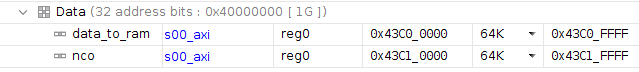
\includegraphics[width=\linewidth]{address}
\caption{Address range used by the IPs as defined by Vivado.}
\label{addr}
\end{figure}

\section{On the Redpitaya ...}

For communicating with the NCO to configure its frequency, we will benefit from an existing 
library function as implemented in {\tt liboscimp\_fpga}. The NCO configuration function
is defined in ``nco\_conf.h'' and requires as argument the {\tt /dev} entry as defined
in the module generator configuration file, the sampling rate $f_{ck}$, the NCO rate 
$f_o$, and the accumulator size $acc$ since as in a DDS, the configuration word is 
$f_o/f_{ck}\times 2^{acc}$.

\lstinputlisting[language=C]{./app/main.c}
%\begin{lstlisting}[language=C]
%#include <stdio.h>
%#include <stdint.h>
%#include <fcntl.h>
%#include <unistd.h>
%#include "nco_conf.h" // liboscimp functions
%
%#define channels 12         // 3 complex short = 6*2*2 bytes/measurement
%
%int main()
%{char c[4096*channels];
% int fi,fo;
% fi=open("/dev/data1600",O_RDWR);
% fo=open("/tmp/data.bin",O_WRONLY|O_CREAT,0666);
% nco_counter_send_conf("/dev/datanco0", 125000000, 10000000, 32, 0,   1,   1);
%                     // /dev            f_ck=125M  f_o=10M  acc offs pinc poff
% read(fi,c,4096*channels);  // 4096 elements of channels bytes each
% write(fo,c,4096*channels);
% close(fi);
% close(fo);
%}
%\end{lstlisting}

\begin{figure}[h!tb]
\begin{center}
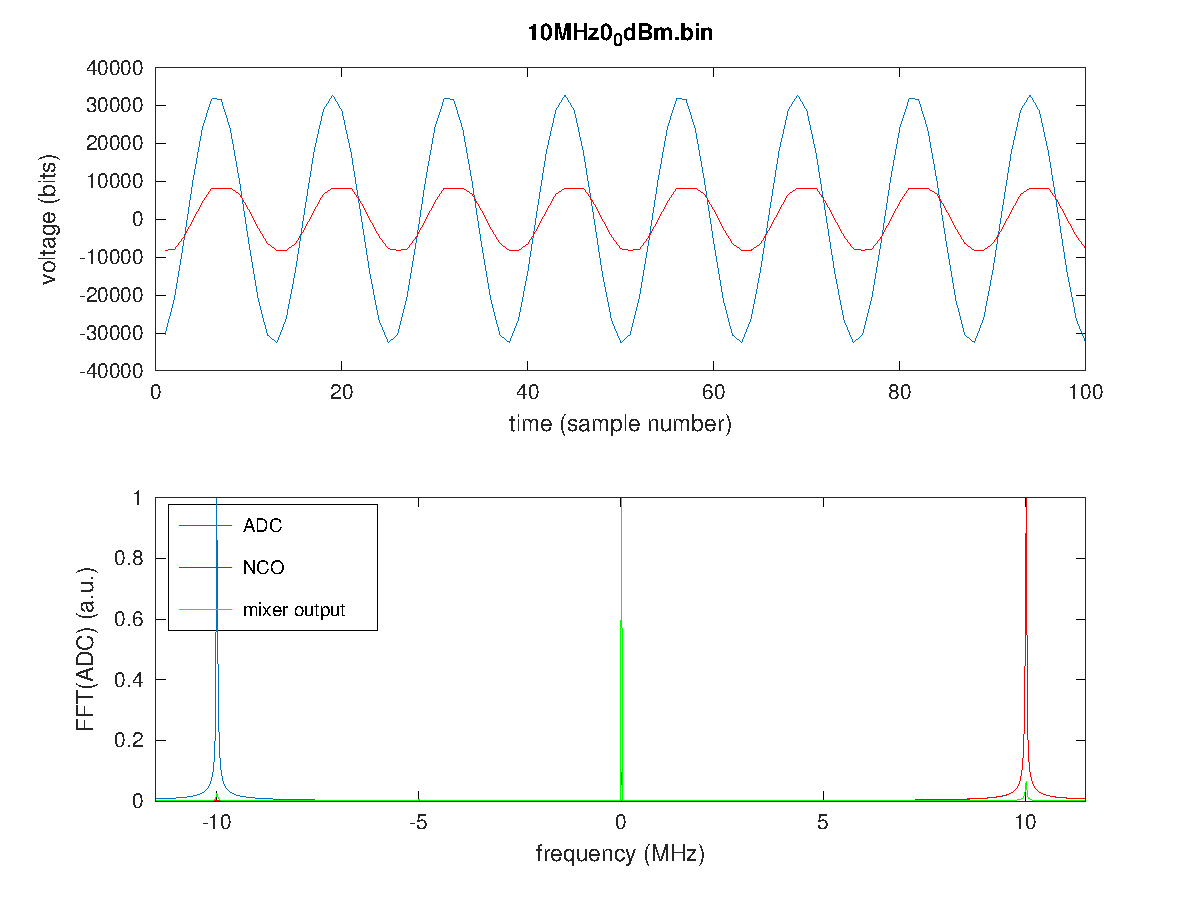
\includegraphics[width=.49\linewidth]{10MHz0_0dBm.pdf}
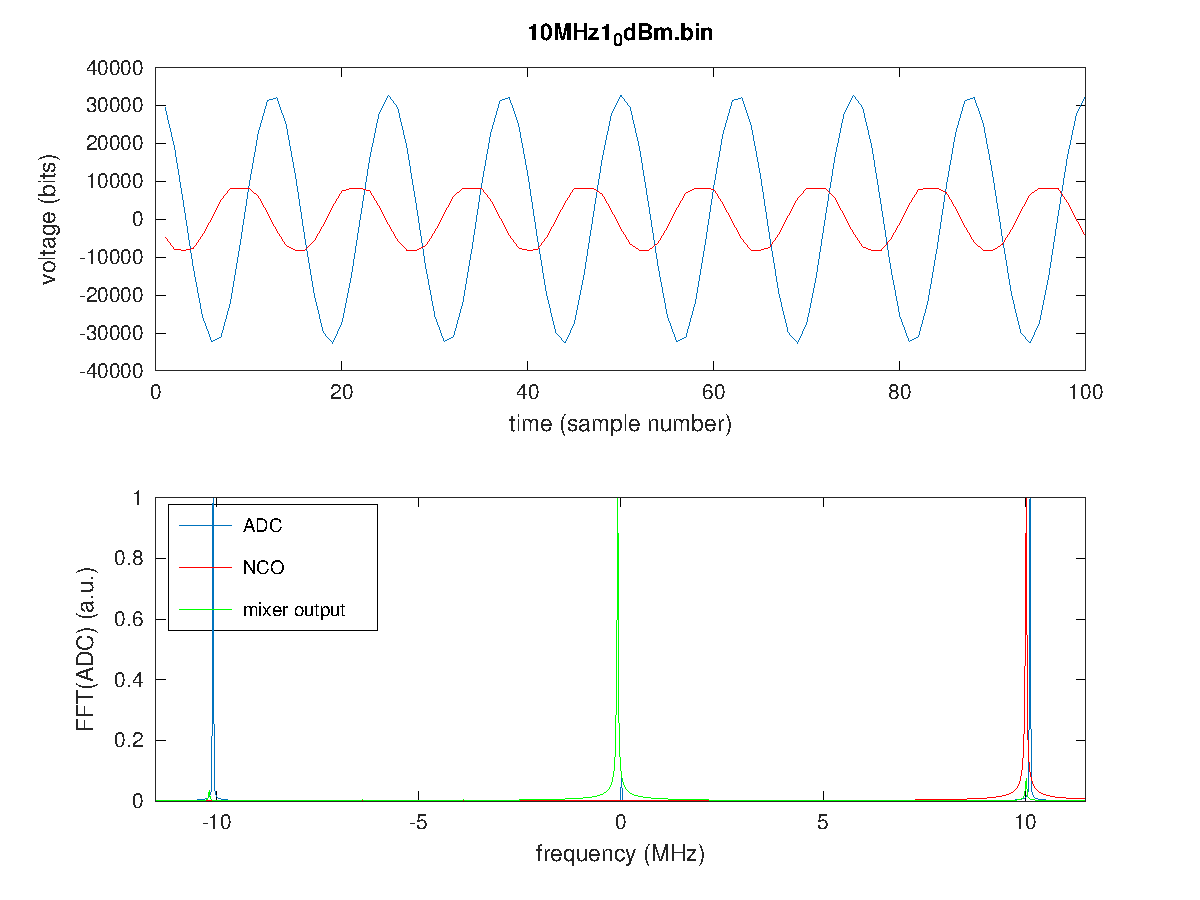
\includegraphics[width=.49\linewidth]{10MHz1_0dBm.pdf}

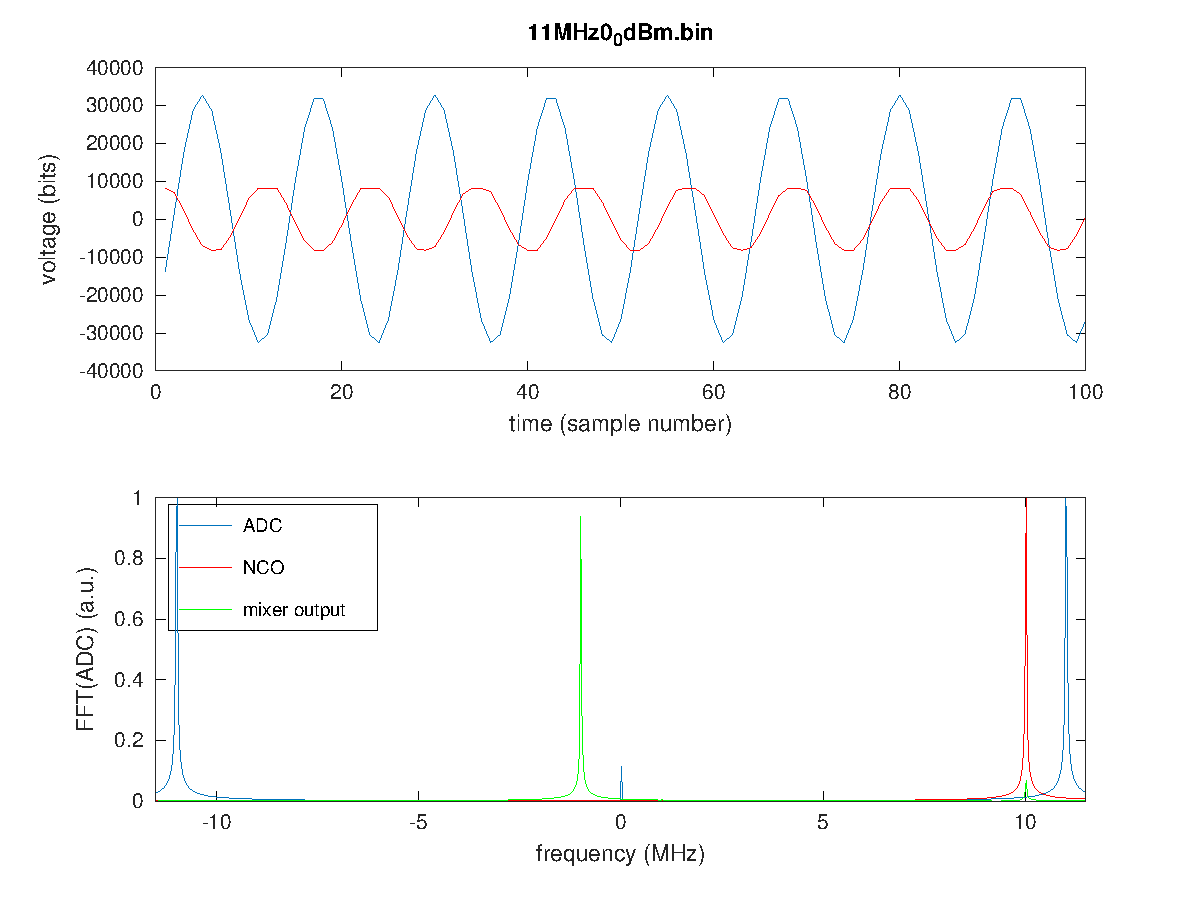
\includegraphics[width=.49\linewidth]{11MHz0_0dBm.pdf}
\end{center}
\vspace{-0.5cm}
\caption{Left to right: 10.0~MHz input signal, 10.1~MHz input signal, and 11.0~MHz input signal.
Each chart exhibits (top) the time domain acquisition (ADC) and local oscillator (NCO) real part,
and (bottom) the frequency domain Fourier transform of the ADC, NCO and mixer output.}
\label{fir}
\end{figure}
\end{document}
